\documentclass{moncours}
\usepackage{minted}
\usepackage{float}
%\usepackage{pygmentize}




\makeindex




\begin{document}

\newcounter{tmp} % pour couper les boîtes énoncés au milieu d'un enumerate

\renewcommand{\labelitemi}{\textbullet}
\renewcommand{\labelitemii}{$\circ$} 

\frontmatter

\titlePage[./images/couvertureFlo3e_v1]{Informatique 3\up{e}}{Fiches MITIC}{Institut Florimont}{Petit-Lancy (Suisse)\\ \textcopyright\ Tout droit réservé. Crédit photographie couverture : Institut Florimont. Illustration des premières pages de chapitre issue de \emph{Codex Leicester} de Leonardo da Vinci (domaine public). \\1\up{ère} édition, v1.0 \\ juin 2021} 

% TOC
\pagestyle{empty} % No headers

\tableofcontents % Print the table of contents itself
\cleardoublepage % Forces the first chapter to start on an odd page so it's on the right
\pagestyle{fancy} % Print headers again

%\cleardoublepage % on force une page impaire
%\vspace*{1cm}

\section*{Calendrier des différentes activités (4\up{e})}\index{Calendrier des activités}  

\vfill

\begingroup % permet de bloquer le arraystretch à ce groupe seulement
\renewcommand{\arraystretch}{1.2}
\begin{center}
\begin{tabular}{|l|l|c|l|l|}
\hline
\multirow{2}{*}{\textbf{Nom de la fiche}} & \multirow{2}{*}{\textbf{Matière}} & \multirow{2}{*}{\textbf{Page}} & \textbf{Date de} & \textbf{Nom du} \\
 &  &  & \textbf{réalisation} & \textbf{professeur} \\ \hline
%\rowcolor[gray]{0.8}\multicolumn{5}{|l|}{Rentrée scolaire} \\ \hline 
%\emph{La plateforme Flore} & (Titulaire) & \pageref{plateformeFlore} & & \phantom{xxxxxxxxxxxxxxxx}  \\ \hline
%
% avant les vacances d'octobre
%
\rowcolor[gray]{0.8}\multicolumn{5}{|l|}{Avant les vacances d'octobre} \\ \hline
\emph{Tableur : séance 1} & Mathématiques & \pageref{ficheTableur4e1} & & \\ \hline
\emph{Texte : séance 1} & Anglais & \pageref{ficheTexte4e1} & & \\ \hline

\multicolumn{5}{l}{} \\ \hline % saut ligne

%
% avant les vacances de Noël
%
\rowcolor[gray]{0.8}\multicolumn{5}{|l|}{Avant les vacances de Noël} \\ \hline
\emph{Texte : séance 2} & Français & \pageref{ficheTexte4e3} & & \\ \hline
\emph{Scratch : séance 1} & Mathématiques & \pageref{ficheScratch4e1} & & \\ \hline

\multicolumn{5}{l}{} \\ \hline % saut ligne

%
% avant les vacances de février
%
\rowcolor[gray]{0.8}\multicolumn{5}{|l|}{Avant les vacances de février} \\ \hline
\emph{Image : séance 1} & SVT & \pageref{ficheImage4e2} & & \\ \hline


\multicolumn{5}{l}{} \\ \hline % saut ligne

%
% avant les vacances de printemps
%
\rowcolor[gray]{0.8}\multicolumn{5}{|l|}{Avant les vacances de printemps} \\ \hline
\emph{Tableur : séance 2} & Sciences physiques & \pageref{ficheTableur4e2} & & \\ \hline
\emph{Texte : séance 3} & Mathématiques & \pageref{ficheTexte4e2} & & \\ \hline
\emph{Scratch : séance 2} & Mathématiques & \pageref{ficheScratch4e2} & & \\ \hline
%\emph{Son : séance 2} & Anglais & \pageref{ficheSon4e2} & & \\ \hline

\multicolumn{5}{l}{} \\ \hline % saut ligne


%
% avant les vacances d'été
%
\rowcolor[gray]{0.8}\multicolumn{5}{|l|}{Avant les vacances d'été} \\ \hline
\emph{Image : séance 2} & Français & \pageref{ficheImage4e1} & & \\ \hline
\emph{Scratch : séance 3} & Mathématiques & \pageref{ficheScratch4e3} & & \\ \hline

\multicolumn{5}{l}{} \\ \hline % saut ligne


%
% avant la fin du semestre de cours
%
\rowcolor[gray]{0.8}\multicolumn{5}{|l|}{Avant la fin du semestre de cours (pour les cours au semestre)} \\
 \hline %\emph{Tableur : séance 3} & Géographie & \pageref{ficheTableur4e3} & & \\ \hline
\emph{Image : séance 3} & Arts visuels & \pageref{ficheImage4e3} & & \\ \hline
%\emph{Son : séance 1} & Musique & \pageref{ficheSon4e1} & & \\ \hline
\end{tabular}
\end{center}
\endgroup

\vfill

\cleardoublepage % on force une page impaire pour le clavier
\section*{Les touches spéciales du clavier}\index{Clavier}\index{Touches spéciales}

\vfill

\begin{center}
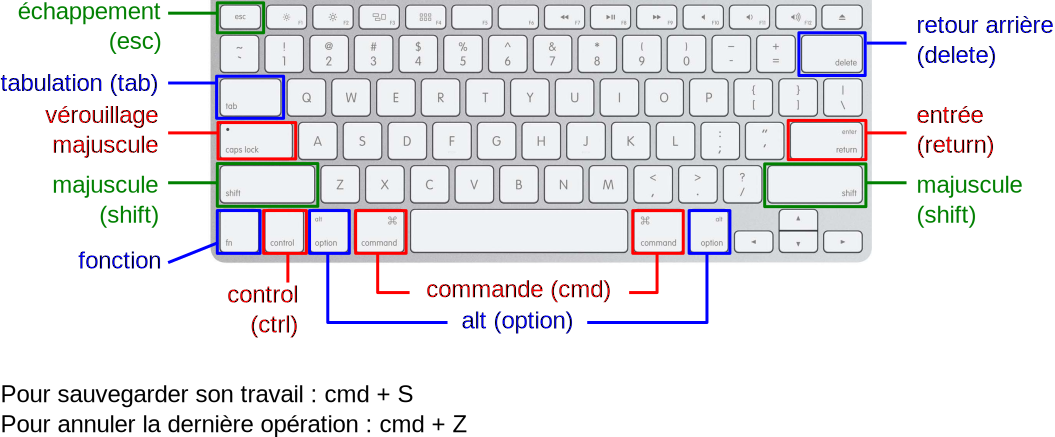
\includegraphics[angle=90,width=.6\textwidth]{./images/generales/clavierTouches}
\end{center}

\vfill

\cleardoublepage % on force une page impaire pour la philosophie du document
\chapter*{Philosophie du document}


\prof{\textbf{ceci est la version professeur du document.} L'icône du professeur est suivie par des informations complémentaires qui n'apparaissent pas dans la version élève.}  

Vous avez entre les mains le deuxième tome d'une série de trois fascicules qui accompagneront les élèves des classes de 6\up{e}, 5\up{e}, 4\up{e} ET 3\up{e} jusqu'au moment où ils recevront un ordinateur qu'ils seront en mesure d'exploiter au mieux pour leur travail.

\vspace{18pt}

Ce document se présente sous la forme d'un livret qui rassemble des fiches MITIC\footnote{MITIC : Médias, Images et Technologies de l'Information et de la Communication.} permettant aux élèves d'apprendre à utiliser les logiciels et espaces numériques mis à leur disposition. Pour l'année de 5\up{e}, sont traités les logiciels \emph{Microsoft Word} (traitement de texte), \emph{Microsoft Excel} (tableur grapheur), \emph{Gimp} (retouche d'image), \emph{Audacity} (traitement des fichiers son) et \emph{Scratch} (programmation). Au début de chaque chapitre un lien permettant de télécharger le logiciel est fourni.

\vspace{18pt}


Chaque fiche est conçue pour être exploitée à plusieurs occasions et dans des matières différentes, à chaque fois lors d'une séance de 45 minutes. La fiche sur le tableur, par exemple, est découverte en physique-chimie (\emph{Séance 1}), exploitée à nouveau en mathématiques (\emph{Séance 2}) puis en histoire-géographie (\emph{Séance 3}) selon un calendrier proposé en début de fiche. Nous avons à chaque fois essayé de faire coïncider les notions abordées dans la fiche avec le programme de la matière concernée.

\vspace{18pt}

Professeurs, c'est à vous que revient la tâche délicate d'inclure le contenu de ces fiches dans votre progression. À vous de le faire vivre : arriver en salle informatique et demander aux élèves de remettre en forme un texte de Molière ne présente que peu d'intérêt pédagogique. Donnez du sens à ces fiches et profitez-en pour diversifier votre enseignement. N'hésitez pas à exploiter dans vos cours les techniques présentées dans ce fascicule afin que les élèves utilisent plusieurs fois leurs nouvelles compétences et, par là-même, les pérennisent.

%\vspace{18pt}

%Ces fiches MITIC sont appelées à évoluer. N'hésitez pas à nous transmettre vos suggestions et nous signaler toute erreur relevée par courriel à l'adresse \texttt{flo-mitic@florimont.ch}.

\vspace{18pt}

Merci d'avance à tous pour votre implication.

\vspace{18pt}

L'équipe de rédaction.

\vspace{2cm}

% \emph{Remarque : il existe une version professeur de ce document, contenant des informations complémentaires, disponible sur l'ENT de l'école.}

  


% Début des chapitres
\setcounter{page}{1} % si on veut forcer la page 1 au début du premier chapitre
\mainmatter
%
  
\begin{minted}{python}
import sympy as sy
\end{minted}

\chapterImage{./images/chapitreVinci4e.png}
%\input{./sources/activite1/activite1.tex}
\chapter{Découverte Python et module Turtle}\index{decouvertePython}

Python est un langage de programmation très implanté dans les milieux éducatif et scientifique de par la clarté de sa grammaire et l'efficacité de son code. Nous allons apprendre dans cette activité à faire le lien entre la programmation Scratch telle que vous l'avez vue en classes de 6\up{ème}, 5\up{ème}, 4\up{ème} et la programmation Python. Cette initiation en douceur à Python va donc vous permettre de découvrir les bases de ce langage. 

\section{Pour bien commencer}

Vous devrez utiliser \emph{Pyzo} pour exécuter votre code Python. \emph{Pyzo} est un éditeur de programme léger permettant d'exécuter du code Python. 

Ouvrir l'éditeur \emph{Pyzo} en cliquant d'abord sur l'icône \includegraphics[width=1cm]{./images/activite7/icone_recherche} puis en complétant la barre de recherche : 

\uneimageici{./images/activite7/recherche_pyzo.png}{.5\textwidth} % reprise image existante

\emph{Pyzo} s'ouvre et vous propose deux zones distinctes de travail :
\begin{itemize}
\item à gauche l'éditeur dans lequel vous allez taper votre code,
\item à droite la console dans laquelle vont apparaître les erreurs de code et les résultats fournis après avoir exécuté le code Python.
\end{itemize}

\uneimageici{./images/activite7/ecran_pyzo.png}{.8\textwidth}% reprise image existante

Commencez par créer un nouveau fichier. Pour cela, sélectionner \texttt{Nouveau} dans le menu \texttt{Fichier}

\uneimageici{./images/activite7/nouveau_fichier.png}{.4\textwidth} % reprise image existante

Puis enregistrez votre fichier au format \texttt{Nom-date.py}

\section{L'activité demandée}



\subsection{Partie Scratch}

En utilisant le logiciel \emph{Scratch}, écrire un script qui dessine un carré.

\uneimageici{./images/activite2/scratch_uncarre.png}{.1\textwidth}

Ecrire ensuite un autre script permettant d'obtenir une suite de trois carrés. 

\uneimageici{./images/activite2/scratch_troiscarres.png}{.3\textwidth}

Par exemple, le code suivant vous permet d'obtenir le résultat escompté

\uneimageici{./images/activite2/codescratch_troiscarres.png}{.2\textwidth}

\subsection{Partie Python}

Nous allons maintenant traduire bloc par bloc en Python le code obtenu dans la première partie.\\

Le bloc suivant

\uneimageici{./images/activite2/scratch_demarrerScript.png}{.15\textwidth}

correspond à l'exécution du code Python sur \emph{Pyzo}

\uneimageici{./images/activite7/executer_fichier.png}{.4\textwidth} % image deja existante

\begin{minted}{python}
from turtle import *
def carre():
color("red")
begin_fill()
for i in range(4}:
down()
forward(50)
left(90)
end_fill()

def ligne():
for i in range(3):
carre()
up()
forward(60)

x = 0
y = 0
for i in range(3):
goto(x, y)
ligne()
x = 0
y = y - 60
\end{minted}
%\newpage

\section{Tracer des courbes et surfaces en Python}\index{courbesPython}

\subsection{Pour bien commencer}

Vous devrez utiliser \emph{Pyzo} pour exécuter votre code Python. \emph{Pyzo} est un éditeur de programme léger permettant d'exécuter du code Python. 

Ouvrir l'éditeur \emph{Pyzo} en cliquant d'abord sur l'icône \includegraphics[width=1cm]{./images/activite7/icone_recherche} puis en complétant la barre de recherche : 

\uneimageici{./images/activite7/recherche_pyzo.png}{.5\textwidth} % reprise image existante

\emph{Pyzo} s'ouvre et vous propose deux zones distinctes de travail :
\begin{itemize}
\item à gauche l'éditeur dans lequel vous allez taper votre code,
\item à droite la console dans laquelle vont apparaître les erreurs de code et les résultats fournis après avoir exécuté le code Python.
\end{itemize}

\uneimageici{./images/activite7/ecran_pyzo.png}{.8\textwidth}% reprise image existante

Commencez par créer un nouveau fichier. Pour cela, sélectionner \texttt{Nouveau} dans le menu \texttt{Fichier}

\uneimageici{./images/activite7/nouveau_fichier.png}{.4\textwidth} % reprise image existante

Puis enregistrez votre fichier au format \texttt{Nom-date.py}



%
%
%  S  É  A  N  C  E     S  U  R     L  E  S     R  A  Y  O  N  S      A  T  O  M  I  Q  U  E  S
%
%

\chapter{Rayon atomique}\label{ficheTableur4e1}

Le but de cette séance est d'utiliser python pour afficher un graphique montrant le rayon atomique en fonction du numéro de l'atome correspondant.

\section{Pour bien démarrer...}

Pour commencer, ouvrez \emph{Excel} et créez un fichier que vous allez exporter au format .CSV en le nommant \texttt{Elements.csv} (Sauvegardez-le tout de suite pour être sûrs de ne pas le perdre par la suite.) Ce fichier contiendra les données que nous allons ensuite afficher sur le graphique. Pendant que vous travaillez, pensez à sauvegarder régulièrement votre travail (raccourci clavier \texttt{Cmd + s}).   

\uneimageici{./images/generales/clavierCmdS}{.4\textwidth}


\section{Sujet de l'activité...}

\boiteEnonceLarge{%

%\vspace{6pt}

Pour compléter le fichier \texttt{Elements.csv}, il faut:

\begin{itemize}
\item Créer les en-têtes du document, nommées \texttt{numéro atomique} et \texttt{rayon atomique (pm)};
\item Remplir la colonne du numéro atomique par les nombres entiers de 1 à 20;
\item Remplir la colonne du rayon atomique par la valeur du rayon atomique associée aux vingt premiers éléments. Pour trouver ces valeurs, une recherche sur internet peut être requise. Assurez-vous que les valeurs soient bien exprimées en picomètres (pm) ou convertissez-les si ce n'est pas le cas.
\end{itemize}
%\vspace{10pt}
} % fin 

\vfill
\phantom{rien}

\boiteEnonceLarge{%
Une fois cela fait, enregistrez le fichier à nouveau. Il va maintenant falloir l'ouvrir grâce à un code python. Vous disposez d'un tel code (mis à votre disposition par votre enseignant) nommé \texttt{$graphique\_rayon\_atomique.py$}. Vérifiez qu'il se trouve bien dans le même dossier que votre fichier \texttt{Elements.csv}.
Lancez le code, il devrait ouvrir une fenêtre avec un graphique tel que présenté ci-dessous.

\uneimageici{./images/activite4/graphique_pre_modif.png}{.6\textwidth}

Certains éléments de ce graphique sont à revoir, vous allez les modifier.

\begin{itemize}
\item Pour commencer, ajoutez l'unité (pm) à l'axe des ordonnées;
\item Ajoutez un titre approprié au graphique en ajoutant une ligne \texttt{plt.title('Titre du graphique')} et en y remplaçant "Titre du graphique" par ce que vous voulez;
\item Modifiez la courbe en remplaçant la couleur par du bleu.
\end{itemize}
\vspace{10pt}
Une fois ces modifications terminées, enregistrez votre code et exécutez-le à nouveau : vous devriez apercevoir une versions à jour du graphique. Si vous essayez de modifier les valeurs du document .csv, vous obtiendrez alors une courbe différente.\\

Maintenant que votre travail est terminé, effectuez un clic droit sur le graphique et enregistrez-le au format PNG (le fichier doit être nommé à partir de votre nom : \texttt{Nom-seance4.png}), puis vous le rendrez sur \emph{Teams} à l'endroit indiqué par votre enseignant (si nécessaire, se reporter à la fiche méthode \emph{Remettre son devoir}, page \pageref{TeamsRemettreDevoir}).
} % fin 

\section{Pour aller plus loin...}
Vous avez modifié un code Python pour personnaliser un graphique, mais on peut faire beaucoup plus!
\begin{itemize}
\item Si vous ajoutez quelques lignes de plus à votre document .csv, que va-t-il se passer?
\item On peut ajouter des colonnes au fichier .csv avec d'autres informations concernant les éléments (masse atomique, électronégativité, etc...) et faire des graphiques similaires, ou même les comparer entre elles. Essayez par exemple de faire un graphique représentant la masse des éléments en fonction de leur numéro atomique;
\item On peut créer plusieurs courbes sur le même graphique pour voir s'il y a des corrélations entre certaines valeurs. Par exemple, vous pouvez tracer la courbe de l'électronégativité en fonction du numéro atomique en plus de celle du rayon atomique et voir s'il y a un point commun entre ces courbes ou non;
\item Modifier l'aspect de la courbe en ajoutant par exemple {plt.rcParams['lines.linestyle'] = '--'}. Cette ligne peut être modifiée pour afficher la courbe sous d'autres formes;
\item Ajouter un affichage des points en plus de la courbe pour une lecture plus claire des résultats..
\end{itemize}

\vfill

%\cadre{Pensez à sauver régulièrement votre travail en appuyant sur \texttt{Cmd + S} ou à partir du menu \texttt{Fichier} en choisissant \texttt{Enregistrer}.

%\uneimageici{./images/generales/clavierCmdS}{.5\textwidth}
%}


%\input{./sources/activite5/activite5.tex}
%\input{./sources/activite6/activite6.tex}
\chapter{Factorisation et développement}\index{factorisationDeveloppement}

Vous avez appris à factoriser et développer des expressions mathématiques. C'est parfois difficile mais cela vous permet de résoudre certains problèmes dont vous ne pourriez trouver la solution autrement. Le langage Python permet d'obtenir un résultat similaire à moindre effort si on sait l'utiliser correctement. Savoir utiliser cet outil pour trouver vos résultats ou vérifier votre travail est une donc compétence bien utile que vous allez apprendre aujourd'hui.\\

\section{Pour bien commencer...}

Vous devrez utiliser \emph{Pyzo} pour exécuter votre code Python. \emph{Pyzo} est un éditeur de programme léger permettant d'exécuter du code Python. 

Ouvrir l'éditeur \emph{Pyzo} en cliquant d'abord sur l'icône \includegraphics[width=1cm]{./images/activite7/icone_recherche} puis en complétant la barre de recherche : 

\uneimageici{./images/activite7/recherche_pyzo.png}{.5\textwidth}

\emph{Pyzo} s'ouvre et vous propose deux zones distinctes de travail :
\begin{itemize}
\item à gauche l'éditeur dans lequel vous allez taper votre code,
\item à droite la console dans laquelle vont apparaître les erreurs de code et les résultats fournis après avoir exécuté le code Python.
\end{itemize}

\uneimageici{./images/activite7/ecran_pyzo.png}{.8\textwidth}



Commencez par créer un nouveau fichier. Pour cela, sélectionner \texttt{Nouveau} dans le menu \texttt{Fichier}

\uneimageici{./images/activite7/nouveau_fichier.png}{.4\textwidth}

Puis enregistrez votre fichier au format \texttt{Nom-activite7.py}


\section{L'activité demandée}

%\vspace{12pt}

\subsection{Etape 1 - calcul manuel}

\vspace{12pt}

\boiteEnonceLarge{% début énoncé étape 1
Dans un premier temps, soyez courageux et effectuez les calculs suivants à la main, afin de comparer plus tard vos résultats et ceux de l'ordinateur.\\

\emph{Exercice 1}\\

Factoriser l'epression suivante : $A=(x-1)(2x+7)+3(1-x)(5-x)$\\

\emph{Exercice 2}\\

Développer l'expression suivante : $B=5(2x-7)(3-x+x^2)$\\

\emph{Exercice 3}\\

Simplifier l'expression suivante : $C=\frac{144x^2+84}{8}$\\

\emph{Exercice 4}\\

Résoudre l'équation suivante : $(9-x^2)(3x-1)=4(x-3)(2x+5)$
}% fin énoncé étape 1

\subsection{Etape 2 - Python}

\vspace{12pt}



\boiteEnonceLarge{% début énoncé
Pour exécuter les codes ci-dessous, vous pouvez sélectionner \texttt{Démarrer le script} dans le menu  \texttt{Exécuter}

\uneimageici{./images/activite7/executer_fichier.png}{.4\textwidth}

Nous allons maintenant retrouver les résultats précédents en utilisant des codes simples du langage Python.\\

En Python, le calcul littéral nécessite l'importation d'un module appelé \texttt{sympy}, puis l'affectation de symboles formels \emph{x, y, z, ...} aux différentes variables \texttt{x, y, z, ...}.\\

 Pour cela, commencez votre code par

\uneimageici{./images/activite7/codePython1.png}{.4\textwidth}

\emph{Exercice 1}\\

Pour factoriser une expression \texttt{E}, \texttt{sympy} utilise \texttt{factor(E)}.\\

Par exemple, on sait que $(x-1)(x+2)+(x-1)(x+3)=(x-1)(2x+5)$. Essayez donc dans votre fenêtre \emph{Pyzo} l'instruction Python suivante pour retrouver ce résultat.

\uneimageici{./images/activite7/codePython2.png}{.6\textwidth}

Vous remarquerez qu'en Python, les produits s'expriment avec \texttt{*} \\

Essayez maintenant d'obtenir à l'aide de Python le résultat que vous aviez trouvé manuellement pour l'exercice 1.
}%fin énoncé

\boiteEnonceLarge{% debut enonce
\emph{Exercice 2}\\

Pour développer une expression \texttt{E}, \texttt{sympy} utilise \texttt{expand(E)}.\\

Par exemple, on sait que $(x-1)(x-2)=x^2-3x+2$. Essayez donc dans votre fenêtre \emph{Pyzo} l'instruction Python \\

\texttt{print(expand((x-1)*(x-2)))}  \\

pour retrouver ce résultat.\\

Essayez maintenant d'obtenir à l'aide de Python le résultat que vous aviez trouvé manuellement pour l'exercice 2.\\



\emph{Exercice 3}\\

Pour simplifier une expression \texttt{E}, \emph{sympy} utilise \texttt{simplify(E)}.\\

Par exemple, on sait que pour $x\ne0$, on peut écrire $\frac{2x^2+6x}{2x}=x+3$. Essayez donc dans votre fenêtre \emph{Pyzo} l'instruction Python \\

\texttt{print(simplify(2*x**2+6*x)/(2*x))}  \\

pour retrouver ce résultat. \\

Vous remarquez qu'en Python, les puissances peuvent s'exprimer avec \texttt{**} \\ 

Essayez maintenant d'obtenir à l'aide de Python le résultat que vous aviez trouvé manuellement pour l'exercice 3.\\

\emph{Exercice 4}\\

Pour résoudre une équation  \texttt{E}, \emph{sympy} utilise \texttt{solve(E, x)}.\\

Par exemple, on sait que la solution de l'équation $3x+2=0$ est $-\frac{2}{3}$. Essayez donc dans votre fenêtre \emph{Pyzo} l'instruction Python \\

\texttt{print(solve(3*x+2, x))}  \\

pour retrouver ce résultat.\\

Essayez maintenant d'obtenir à l'aide de Python le résultat que vous saviez trouvé manuellement pour l'exercice 4.
} % fin énoncé

\boiteEnonceLarge{% debut enonce
Une fois les vérifications terminées, vous enregistrerez votre fichier au format PY (le fichier doit être nommé à partir de votre nom : \texttt{Nom-date.py}), puis vous le rendrez sur \emph{Teams} à l'endroit indiqué par votre enseignant (si nécessaire, se reporter à la fiche méthode \emph{Remettre son devoir}, page \pageref{TeamsRemettreDevoir}).
} % fin ennonce


\section{Pour aller plus loin...}

On peut également factoriser et développer des expressions mathématiques, dans le module \emph{Calcul littéral} du logiciel \emph{Geogebra}. Cette méthode ne nécessite pas l'utilisation de code car \emph{Geogebra} s'exécute en utilisant une interface graphique, et bien qu'elle s'avère plus intuitive, elle est aussi plus limitée dans son utilisation.








%\input{./sources/activite8/activite8.tex}
%\input{./sources/activite9/activite9.tex}
%\input{./sources/activite10/activite10.tex}
%\input{./sources/activite11/activite11.tex}
\documentclass{article}
\usepackage[utf8]{inputenc}
\usepackage{graphicx}
\usepackage{wrapfig}
\usepackage{caption}


\begin{document}

\section{Connexion à Office 365 et Teams}

Nikolai

Possibilité de télécharger l'application

\section{Apparence de la page d'accueil}

La page d'accueil de Teams se présente sous forme d'une liste de classes 

\begin{figure}[h]
\includegraphics[width=5cm]{accueil_liste.png}
\centering
\end{figure}

ou sous forme d'une grille de classes \newpage

\begin{figure}[h]
\includegraphics[width=10cm]{accueil_grille.png}
\centering
\end{figure}

Pour passer d'une forme à l'autre, il faut cliquer sur le sigle \includegraphics[width=0.7cm]{bouton_parametres.png}, choisir \textit{Changer d'affichage} dans le menu déroulant, comme dans l'exemple illustré ci-dessous :

\begin{figure}[h]
\includegraphics[width=10cm]{changement_liste.png}
\centering
\end{figure}

il faut ensuite sélectionner le type d'affichage souhaité entre \textit{Grille} et \textit{Liste}
\newpage

\begin{figure}[h]
\includegraphics[width=12cm]{choix_parametre.png}
\centering
\end{figure}

 Pour entrer maintenant dans votre classe, dans la matière de votre choix, il suffit de cliquer sur l'icône correspondante

\begin{figure}[h]
\includegraphics[width=12cm]{entree_classe.png}
\centering
\end{figure}

\newpage

\section{Utilisation de la messagerie}

La messagerie instantanée proposée par Teams doit permettre aux élèves et aux enseignants de communiquer en dehors de l'école dans un cadre qui reste strictement scolaire. Ainsi les messages personnels n'ont aucune raison d'être sur Teams. Il n'est par ailleurs pas possible pour un élève de supprimer un message envoyé. Seul le modérateur de la classe peut procéder à une telle suppression. 

Par ailleurs, toute forme d'insulte, de jugement personnel ou de critique envers un membre de la classe est à proscrire.



\section{Consulter et télécharger un document}

Nikolai

\section{Déposer un devoir}

Pour consulter les devoirs déposés par votre enseignant, il faut choisir \textit{2 de plus} dans la barre de menus du haut de page, puis sélectionner \textit{Devoirs}.

\begin{figure}[h]
\includegraphics[width=10cm]{devoir1.png}
\centering
\end{figure}

La page qui s'affiche maintenant fait le bilan de ce qui a déjà été fait et des devoirs proposés par votre enseignant. En cliquant sur \textit{Rédaction} vous pourrez accéder au devoir.

\begin{figure}[h]
\includegraphics[width=10cm]{devoir2.png}
\centering
\end{figure}

\newpage
 Vous obtenez alors l'écran suivant

\begin{figure}[h]
\includegraphics[width=12cm]{devoir3.png}
\centering
\end{figure}

Il est maintenant possible de consulter le sujet sous forme de pièce jointe en sélectionnant ...

\section{Accéder à mon carnet}

\section{Rejoindre une visio-conférence}


\end{document}




\section{Séance 1 - utilisation de Geogebra pour construire la droite d'Euler}

construction de médianes, médiatrices, hauteurs, bissectrices, droite d'Euler et cercle d'Euler à partir d'un triangle (Geogebra a déjà été utilisé au cycle) - activité déjà créée\\

matière mathématiques

\section{Séance 2 - découverte Python et module turtle}

découverte de Python par comparaison avec les modules Scratch utilisés au cycle. Utilisation du module Turtle en Python pour créer une répétition de carrés - activité déjà créée\\

matière mathématiques

\section{Séance 22 - découverte Python sur les variables et conditions}

passage de Scratch à Python\\

matière mathématiques

\section{Séance 3  - dessin d'une courbe en Python}

découverte des courbes et surfaces en Python (2D, 3D), changement de couleurs, d'épaisseur de trait, de type de trait. Les codes sources sont donnés aux élèves - activité déjà créée\\

matière mathématiques

\section{Séance 4 - expérience physique et courbes en Python}

 à partir d'une expérience physique, recherche d'informations sur Internet, création d'un fichier csv sur Excel, vérification que le fichier respecte des normes, création d'une courbe Python à partir de ce fichier, ajout de l'unité à un axe et changement de couleur de courbe - activité en cours de création par Nikolai\\

matière sciences physiques

\section{Séaence 5 - résistivité Sebastien Perrad}

à partir de résultats obtenus en physique sur la résistivité, calcul d'un coefficient puis placement des solutions dans un fichier Excel afin de tracer une courbe à partir d'Excel. - activité proposée par Sebastien Perrad, un peu plus difficile que ce que les élèves font au cycle.\\

matière sciences physiques

\section{Séance 6 - de traitement de l'image avec Python}

utilisation des filtres pour tranformer une photo en Python. traitement d'une image en Python, (contraste, luminosité, pixels). Les codes sources sont fournis à l'élève - activité non réalisée\\

 matière dessin ou mathématiques

\section{Séance 7 - calcul littéral - factorisation, développement}

activité 7 : apprendre à factoriser et développer en Python pour vérifier des résultats trouvés manuellement en cours de maths - activité déjà créée et testée en classe. L'activité est assez facile, mais le chapitre sur la factorisation est une bête noire pour les élèves\\

matière mathématiques


\section{Séance 8 - utilisation des moteurs de recherches - social dilemma}

expérience de groupe pour comprendre la réponse fournie par les moteurs de recherche en fonction des recherches antérieures effectuées. Connaissance du mode de rémunération des Gafam et du traitement de l'information. Sensibilisation à l'origine de l'information sur Internet - activité non réalisée.\\

matière Histoire


\section{Séance 9 - statistique descriptive avec Excel}

utilisation de Excel pour les statistiques descriptives (pouvant servir d'appui au programme de maths) - activité non réalisée\\

matière mathématiques

\section{Séance 10 - statistique descriptive avec Python}

utilisation de Python pour les statistiques descriptives (pouvant servir d'appui au programme de maths) - activité non réalisée\\

matière mathématiques

\section{Séance 11 - création site Web avec WordPress}

création d'un site web avec WordPress (prélude à la création d'une page web en Python pour les élèves de seconde bac) - activité non réalisée. site relatif à un événement historique en relation avec le programme d'histoire ou d'économie\\

matière histoire ou économie










\printindex % il faut utiliser en console "makeindex monfichier.idx" pour faire afficher l'index

\end{document}


